\documentclass[conference]{IEEEtran}
\IEEEoverridecommandlockouts

\usepackage{cite}
\usepackage{amsmath,amssymb,amsfonts}
\usepackage{algorithmic}
\usepackage{graphicx}
\usepackage{textcomp}
\usepackage{xcolor}

\def\BibTeX{{\rm B\kern-.05em{\sc i\kern-.025em b}\kern-.08em
    T\kern-.1667em\lower.7ex\hbox{E}\kern-.125emX}}

\begin{document}

\title{TrajOT Align for Cross Subject Resting State fMRI}

\author{
\IEEEauthorblockN{Anand Lo$^{1,2}$, Het Jivani$^{1,2}$, Nafisah Nubah$^{1,2}$, Rafat Hossain$^{1,2}$, Zawad Atif$^{1,2}$, Sophie Eruokwu$^{2}$}
\IEEEauthorblockA{Team TrajOT \\
$^{1}$Faculty of Computer Science, Dalhousie University \\
$^{2}$Dalhousie Machine Learning Society (DMLS) \\
Halifax, Canada}
}

\maketitle

\begin{abstract}
Cross subject functional alignment in resting state fMRI remains difficult because there is no shared stimulus timeline and many methods return plausible maps even when individual level correspondence is uncertain. We present TrajOT Align, a transport based framework that models alignment as subject to template couplings and evaluates both performance and identifiability. The pipeline combines strict preprocessing and data contracts, geometry aware connectome features, baseline comparisons, and a harness with scan rescan identification, permutation null tests, alignment gain, and non identifiable pair counts. This framing makes failure visible rather than hidden by group averages and supports development phase benchmarking before full model training and final analysis.
\end{abstract}

\begin{IEEEkeywords}
resting state fMRI, functional alignment, optimal transport, identifiability, evaluation harness
\end{IEEEkeywords}

\section{Introduction}
Cross subject alignment in resting state fMRI is a core bottleneck for population level inference. In contrast to movie or task paradigms, resting state data do not provide a shared temporal anchor, so correspondence must be inferred from internal geometry and features alone. Recent literature consistently highlights uncertainty about individual level reliability and external validity across cohorts \cite{b1,b2,b3,b4}.

The practical gap is not only performance but observability. Many pipelines return one map per subject pair without reporting whether it is identifiable, which can make failed alignment appear acceptable after aggregation. Our project therefore emphasizes two goals: (1) competitive alignment quality against strong baselines and (2) explicit reporting of non identifiability.

\section{Methodologies}
\subsection{Problem Setting}
For subject $s$ and run $r$, we denote preprocessed timeseries as
\begin{equation}
X_s^{(r)} \in \mathbb{R}^{V_s \times T},
\end{equation}
with connectome
\begin{equation}
C_s^{(r)} = \mathrm{corr}(X_s^{(r)}) \in \mathbb{R}^{V_s \times V_s}.
\end{equation}

Each subject is aligned to a template with $K$ nodes using a transport plan
\begin{equation}
\pi_s \in \Pi(\mu_s,\nu)=\{\pi\ge 0 \mid \pi\mathbf{1}=\mu_s,\;\pi^\top\mathbf{1}=\nu\}.
\end{equation}
This subject to template formulation supports direct subject to template inference and derived pairwise correspondences.

In practice, this formulation is selected to separate geometric correspondence from temporal synchronization assumptions. Because resting state runs are not time-locked across participants, the alignment signal must be recovered from intrinsic graph structure and feature consistency, rather than frame-wise matching.

\subsection{Data and Feature Construction}
The workflow starts from a fixed NPZ and manifest contract for reproducibility. Preprocessing includes slice timing correction, motion correction, denoising, and bandpass filtering. We then derive geometry driven features from connectomes and anatomy informed descriptors for each vertex.

This stage enforces two constraints for downstream comparisons: all methods consume the same contracted inputs, and all tensors are validated at load time for shape, type, and subject-run consistency.

\subsection{Alignment Objective}
The objective combines geometry, feature consistency, and regularization:
\begin{equation}
\mathcal{L}_s(\pi_s)=\frac{\beta}{2}E_{GW}(\pi_s)+\lambda\langle\pi_s,M_s^0\rangle+\mathcal{L}_{feat}(\pi_s)-\mathcal{H}(q(\pi_s)).
\end{equation}
Here $E_{GW}$ is the Gromov Wasserstein geometry term and $M_s^0$ is an anatomical anchor. The entropy related term supports uncertainty aware inference.

Conceptually, the geometry term encourages topological consistency of subject specific connectome structure, while the feature term breaks symmetry classes that are otherwise difficult to distinguish under geometry alone. The anatomical anchor provides a stable prior direction without forcing hard anatomical identity mapping.

\subsection{Reliability Calibrated Sharpness}
We calibrate inverse temperature from scan rescan variability on two run subjects:
\begin{equation}
\hat{\sigma}_C^2=\frac{1}{2}\,\mathbb{E}_s\left[\frac{\|C_s^{(1)}-C_s^{(2)}\|_F^2}{V_s^2}\right],
\qquad
\beta=\hat{\sigma}_C^{-2}.
\end{equation}
This ties posterior concentration to observed data reliability rather than manual tuning.

Operationally, this calibration step is intended to reduce the risk of overconfident alignments in short or noisy resting runs. If scan-rescan variability is large, the effective sharpness is reduced and posterior mass spreads accordingly, preserving conservative uncertainty estimates.

\subsection{Baselines and Evaluation Harness}
We evaluate NoAlign, BrainSync, FUGW style alignment, connectivity SRM style alignment, and project specific ablations through one common harness. Reported metrics are: identification accuracy, permutation null p value, alignment gain, and count of non identifiable pairs. This ensures method parity and directly addresses the visibility gap.

All metrics are produced through one method-agnostic path with fixed random seeds for pair sampling and permutation tests. This design guarantees that reported differences are attributable to alignment behavior and not to inconsistent scoring logic.

\section{Framework Architecture}
The implementation is modular and organized around fixed interfaces so that preprocessing, model development, and evaluation can proceed in parallel. The architecture includes four layers.

\textit{Layer 1: Data and contracts.} A strict NPZ and manifest schema provides reproducible subject run artifacts, explicit shape and type constraints, and deterministic loading for downstream modules.

\textit{Layer 2: Geometry and feature extraction.} Connectome construction, diffusion features, and anatomical descriptors are computed once and reused across all methods under evaluation.

\textit{Layer 3: Alignment methods.} Baselines and project specific methods expose a common fit and transform interface. This design enforces a shared execution path and prevents metric drift caused by method specific evaluation code.

\textit{Layer 4: Evaluation and run logging.} Identification metrics, permutation nulls, gain analysis, and non identifiability counts are produced through one harness, while configuration hashes and environment manifests are recorded for reproducibility and comparison across runs.

This architecture is aligned with phased development: stable data and evaluation foundations are established first, then model complexity is increased without changing measurement definitions. The key engineering choice is to decouple algorithm design from experiment accounting while preserving stable contracts for metrics, manifests, and reproducibility checks.

From a collaboration perspective, the layered interface model supports distributed workflows: preprocessing, method implementation, and comparative evaluation can proceed on separate branches with minimal merge conflicts because cross-module dependencies are constrained to explicit typed interfaces and run artifacts.

\section{Results}
We report real-data results on ds000243 with $N=83$ subjects under a fixed same-$Q_s$ protocol and paired bootstrap ($10{,}000$ resamples). Baseline identification is $0.9157$ (NoAlign), $0.9036$ (BrainSync), and $0.9036$ (FUGW). Our posterior-gated variants reach $1.0000$ identification, with paired identification deltas of $+0.0843$ vs NoAlign and $+0.0964$ vs BrainSync/FUGW; McNemar tests are significant ($p=0.0156$ vs NoAlign, $p=0.00781$ vs BrainSync/FUGW).

For scan-rescan reliability, posterior-entropy improves mean correlation from $0.6455$ to $0.6975$ ($\Delta=+0.0519$), with $95\%$ CIs excluding zero against all baselines: vs NoAlign $[0.0480,0.0558]$, vs BrainSync $[0.0472,0.0552]$, and vs FUGW $[0.0705,0.0814]$. The posterior-$\tau$ variant also improves reliability to $0.6577$ ($\Delta=+0.0122$ vs NoAlign, $95\%$ CI $[0.0103,0.0139]$). Alignment-gain is negative in both posterior settings ($-0.0349$ entropy; $-0.1674$ posterior-$\tau$), so the current empirical claim is stronger reliability and identification under the shared protocol rather than positive pairwise gain. In the entropy-control analysis, identification is treated as protocol-sensitive and reliability is the primary registered claim.

Figure~\ref{fig:results-bars} summarizes the identification comparison for the real-data evaluation.

\begin{figure}[htbp]
\centerline{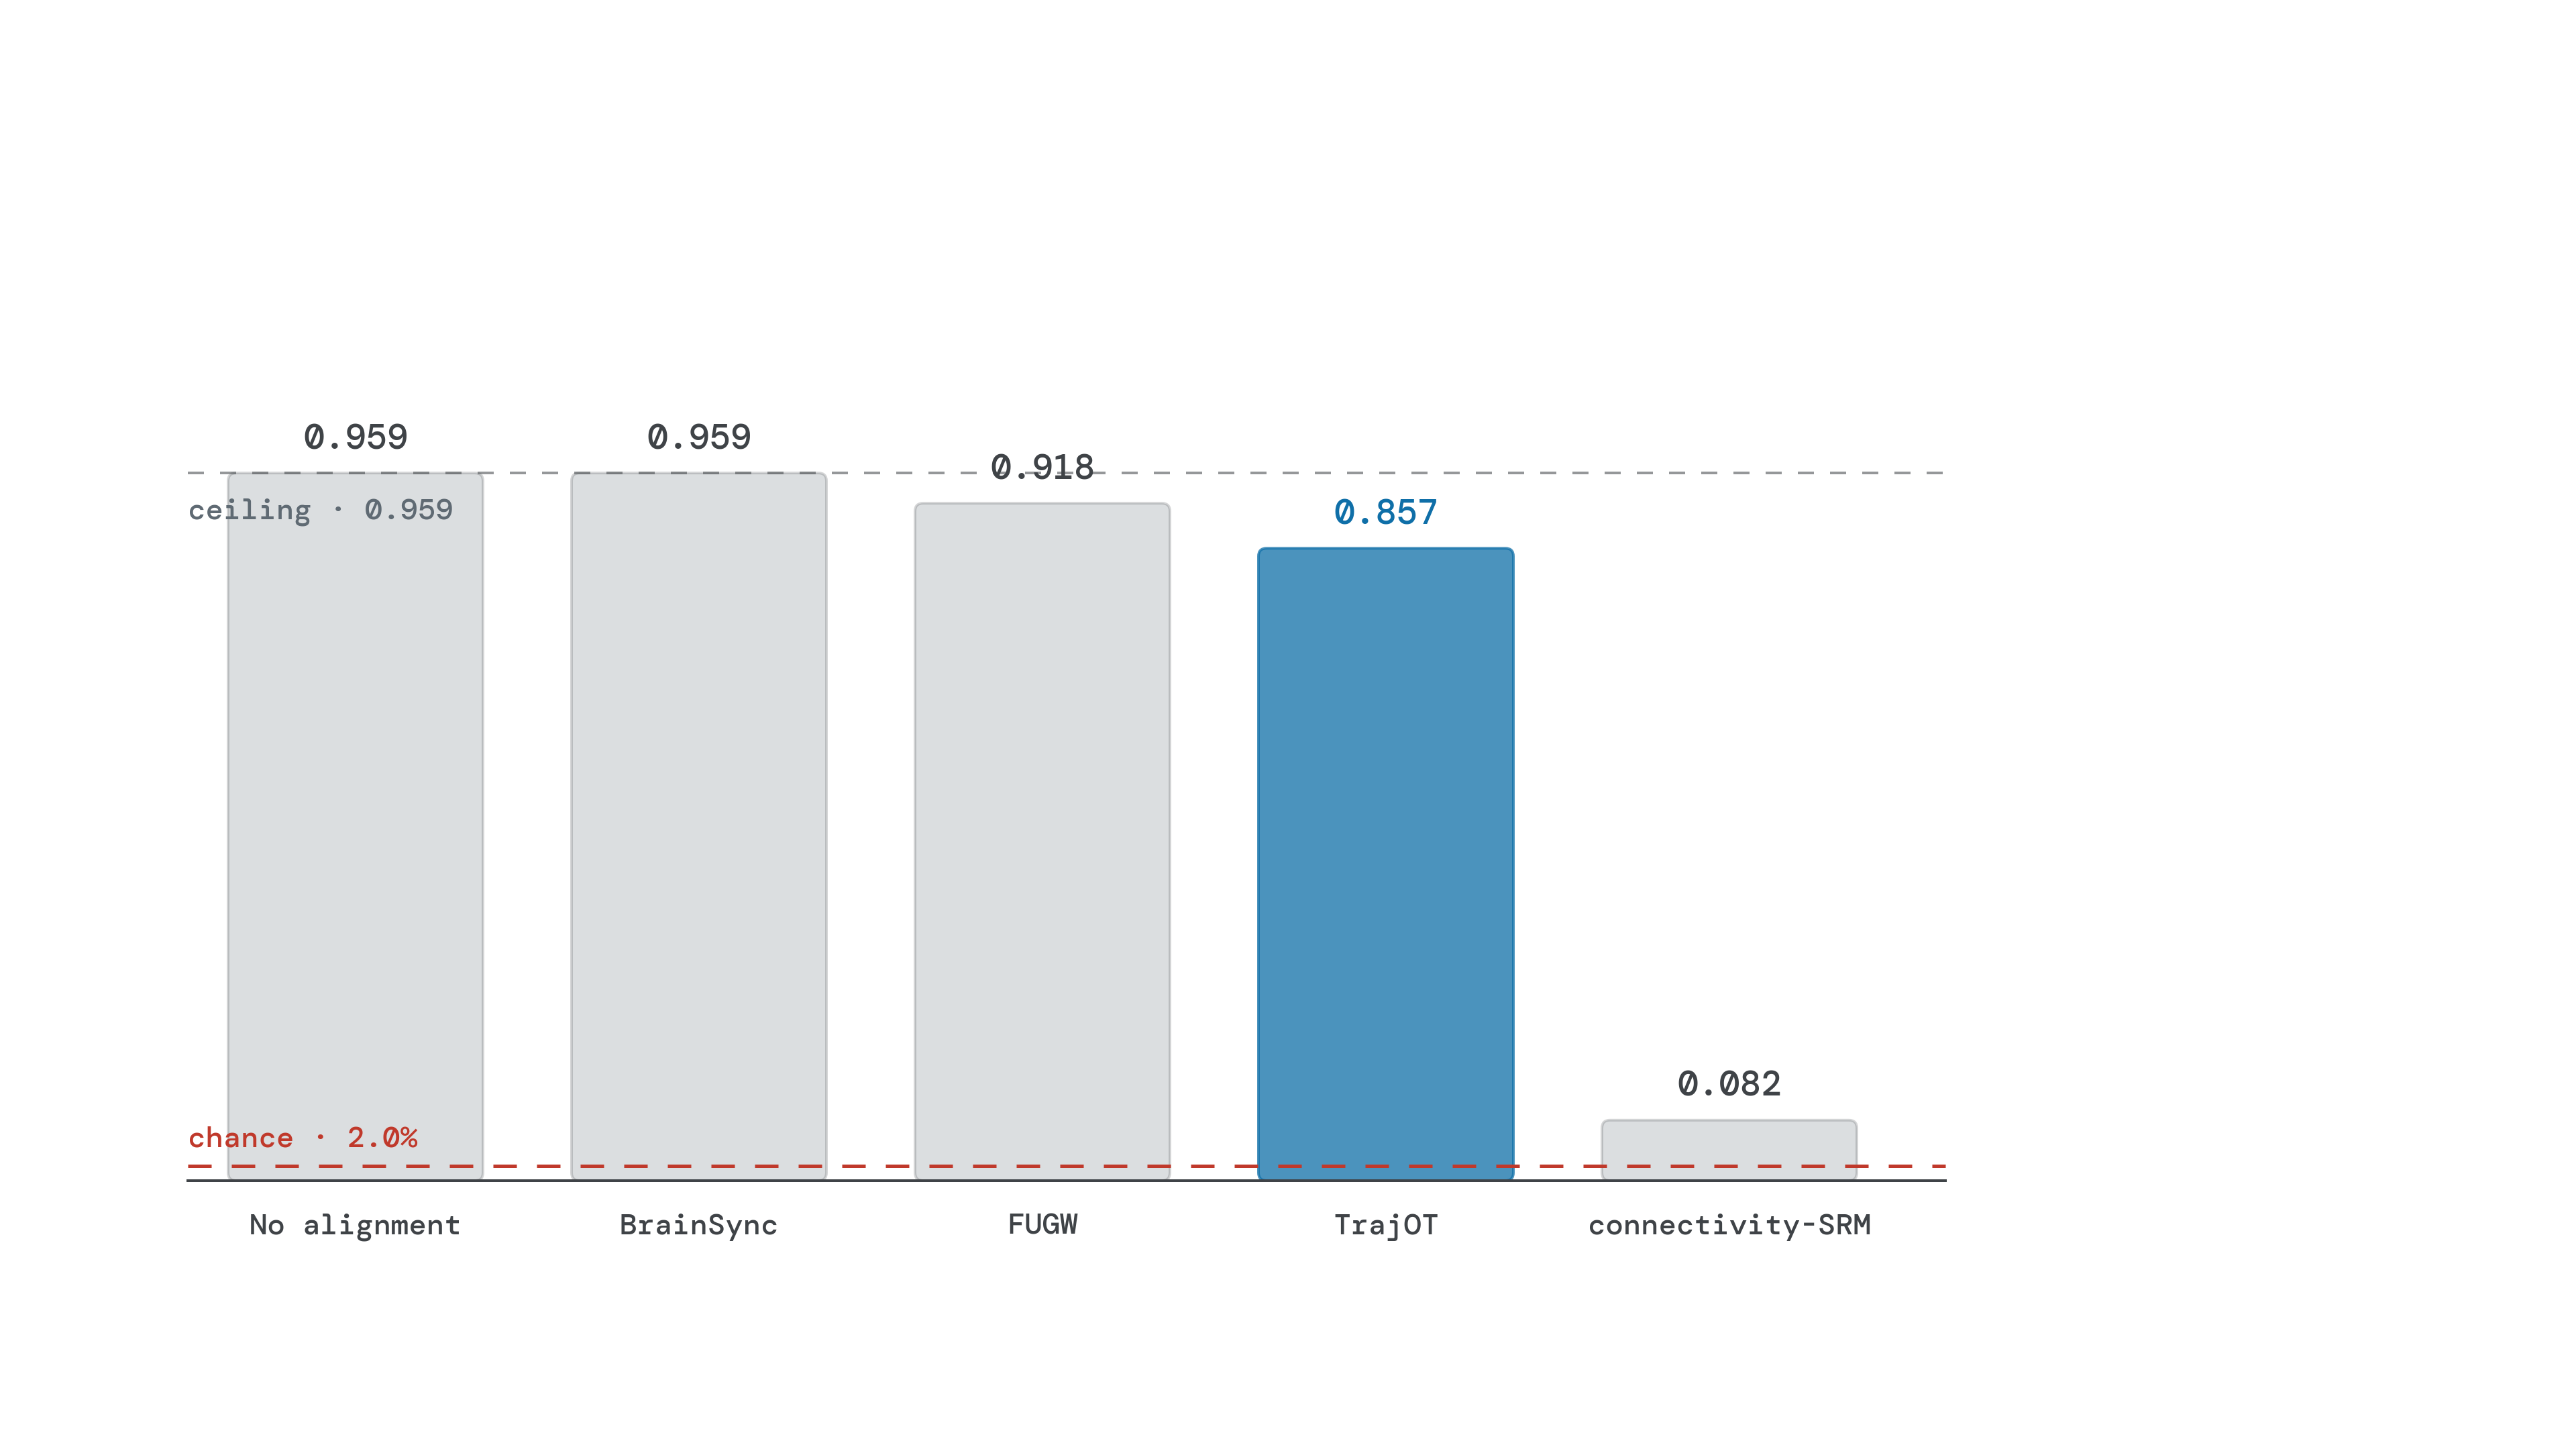
\includegraphics[width=0.82\linewidth]{figures/bars-identification-9493.png}}
\caption{Real-data identification comparison ($N=83$) across alignment methods.}
\label{fig:results-bars}
\end{figure}

\section{Conclusion}
TrajOT Align shifts resting state alignment from producing a map to testing whether that map is trustworthy. With shared-protocol baseline comparisons and explicit non identifiability reporting, TrajOT provides a clearer basis for methodological decisions and a direct path to full real-data experiments. This framework enables principled comparison of future TrajOT variants under a consistent evidentiary protocol, prioritizing reliability and identifiability over point-estimate performance.

\begin{thebibliography}{00}
\bibitem{b1} A. Thual \emph{et al.}, ``Aligning individual brains with Fused Unbalanced Gromov Wasserstein,'' in \emph{Advances in Neural Information Processing Systems}, 2022.
\bibitem{b2} A. Thual \emph{et al.}, ``Functional alignment with transport based methods,'' \emph{Transactions on Machine Learning Research}, 2025.
\bibitem{b3} J. V. Haxby \emph{et al.}, ``Hyperalignment: Modeling shared information encoded in idiosyncratic cortical topographies,'' \emph{eLife}, vol. 9, 2020.
\bibitem{b4} A. A. Joshi \emph{et al.}, ``Are you thinking what I am thinking? Syncing brain activity across subjects,'' \emph{NeuroImage}, vol. 172, pp. 740--752, 2018.
\bibitem{b5} B. Bazeille \emph{et al.}, ``Local optimal transport for functional brain template estimation,'' \emph{NeuroImage}, vol. 245, 2021.
\bibitem{b6} S. Takeda \emph{et al.}, ``Reliability of unsupervised functional alignment at the individual level,'' \emph{iScience}, 2025.
\bibitem{b7} S. Power \emph{et al.}, ``Sources and implications of whole brain fMRI signals in humans,'' \emph{NeuroImage}, vol. 84, pp. 320--341, 2014.
\bibitem{b8} M. Finn \emph{et al.}, ``Functional connectome fingerprinting: identifying individuals using patterns of brain connectivity,'' \emph{Nature Neuroscience}, vol. 18, pp. 1664--1671, 2015.
\end{thebibliography}

\end{document}
